\documentclass[12pt]{article}
\usepackage{fullpage}

\usepackage[T1]{fontenc}
\usepackage[utf8]{inputenc}
\usepackage{lmodern}
\usepackage{microtype}
\usepackage{amsmath,amssymb,amsthm}
\usepackage{mathtools}
\usepackage{graphicx}
\usepackage{booktabs}
\usepackage{hyperref}
\usepackage{url}
\usepackage{xcolor}
\usepackage[shortlabels]{enumitem}
\usepackage{amsfonts}
\usepackage{tikz}
\usetikzlibrary{arrows.meta,positioning,shapes.geometric,calc,patterns,decorations.pathreplacing}
\usepackage[ruled,vlined,linesnumbered]{algorithm2e}

\hypersetup{colorlinks=true,linkcolor=blue,citecolor=blue,urlcolor=blue}

\theoremstyle{plain}
\newtheorem{theorem}{Theorem}
\newtheorem{proposition}[theorem]{Proposition}
\newtheorem{lemma}[theorem]{Lemma}
\newtheorem{corollary}[theorem]{Corollary}

\theoremstyle{definition}
\newtheorem{definition}[theorem]{Definition}

\theoremstyle{remark}
\newtheorem*{remark}{Remark}
\newtheorem*{observation}{Observation}

\newcommand{\eps}{\varepsilon}
\newcommand{\R}{\mathbb{R}}
\newcommand{\E}{\mathbb{E}}
\newcommand{\Tr}{\mathrm{tr}}
\newcommand{\Reff}{R_{\mathrm{eff}}}

\title{Partial Solution to Problem 6 --- Existence of $\eps$-Light Subsets\\[6pt]
\large A submission to the First Proof challenge}

\author{
  Mark Dillerop\footnote{Email: dillerop@gmail.com}\\
  \textit{Independent / Ars Socratica}
}

\date{February 12, 2026}

\begin{document}
\maketitle

\begin{abstract}
We study Problem~6 from the First Proof challenge \cite{FirstProof}, posed by Daniel Spielman: does every graph $G$ on $n$ vertices admit an $\eps$-light subset $S$ (meaning $L_S \preceq \eps L$) of size $|S| \geq c\eps n$ for some universal constant $c > 0$? We establish the optimal upper bound $c \leq 1/2$ (Proposition~\ref{prop:upper}), prove the conjecture for complete graphs with $c = 1/2$ (Theorem~\ref{thm:complete}), and develop a log-det multi-bin barrier method. We prove that the partition approach with $k = \lceil 2/\eps \rceil$ bins \emph{cannot} achieve $c = 1/2$ for all graphs: the barbell graph provides a counterexample where the barrier blows up (Proposition~\ref{prop:barbell}). However, with $k = \lceil 3/\eps \rceil$ bins, the greedy achieves $\mu_{\max} \leq 2/3$ computationally for all tested graph families, targeting $c = 1/3$. The general conjecture remains open; we precisely characterize the remaining gap and document why standard spectral tools are insufficient.
We conjecture the answer is \textbf{YES} with optimal constant $c = 1/2$, supported by extensive computational evidence. The partition approach can provably achieve at most $c = 1/3$; achieving $c = 1/2$ requires a non-partition method.
\end{abstract}

\tableofcontents
\newpage

%======================================================================
\section{Problem Statement}\label{sec:problem}
%======================================================================

The following is Problem~6 from the First Proof challenge \cite{FirstProof}, authored by Daniel Spielman (Yale University).

\medskip

\noindent\textbf{Problem 6.} \textit{For a graph $G = (V, E)$ with $n = |V|$ and Laplacian $L$, the induced subgraph Laplacian is $L_S = \sum_{\{u,v\} \in E(S,S)} L_{uv}$. A set $S \subseteq V$ is $\eps$-light if $L_S \preceq \eps L$. Does there exist a universal constant $c > 0$ such that for every graph $G$ and every $\eps \in (0,1)$, there exists an $\eps$-light subset $S$ with $|S| \geq c\eps n$?}

\medskip

\noindent\textbf{Our answer: conjecturally YES}, with optimal constant $c = 1/2$. Via the partition approach, we target $c = 1/3$ (the barbell graph obstructs $c = 1/2$ via partitions).

%======================================================================
\section{Normalized Formulation}\label{sec:normalized}
%======================================================================

Let $\Pi$ denote the orthogonal projector onto $\mathbf{1}^\perp$ and define $\tilde{M} := L^{+/2} M L^{+/2}$ for any symmetric matrix $M$, where $L^+$ is the Moore--Penrose pseudoinverse of $L$.

\begin{lemma}[Normalization]\label{lem:norm}
$L_S \preceq \eps L$ if and only if $\|\tilde{L}_S\| \leq \eps$, where $\|\cdot\|$ denotes the spectral norm restricted to $\mathbf{1}^\perp$. The normalized edge Laplacians $\tilde{L}_{uv}$ are rank-1 PSD with $\|\tilde{L}_{uv}\| = \Tr(\tilde{L}_{uv}) = \Reff(u,v)$, and $\sum_{e \in E} \tilde{L}_e = \Pi$.
\end{lemma}

\begin{proof}
$\tilde{L}_{uv} = L^{+/2}(\mathbf{e}_u - \mathbf{e}_v)(\mathbf{e}_u - \mathbf{e}_v)^\top L^{+/2}$ is rank-1 PSD. Its trace is $(\mathbf{e}_u - \mathbf{e}_v)^\top L^+ (\mathbf{e}_u - \mathbf{e}_v) = \Reff(u,v)$. For rank-1 PSD matrices, $\|\cdot\| = \Tr(\cdot)$. Summing over all edges: $\sum_e \tilde{L}_e = L^{+/2} L L^{+/2} = \Pi$.
\end{proof}

%======================================================================
\section{Proved Results}\label{sec:results}
%======================================================================

\subsection{Linearization}

\begin{lemma}[Linearization]\label{lem:linear}
For any $S \subseteq V$: $L_S \preceq \frac{1}{2}\sum_{v \in S} L_v^*$, where $L_v^* = \sum_{u \sim v} L_{uv}$ is the star Laplacian of $v$.
\end{lemma}

\begin{proof}
For indicators $s_u, s_v \in \{0,1\}$: $s_u s_v \leq \frac{1}{2}(s_u + s_v)$. Since $L_{uv} \succeq 0$:
\[
L_S = \sum_e s_u s_v L_{uv} \preceq \sum_e \tfrac{s_u + s_v}{2} L_{uv} = \tfrac{1}{2}\sum_{v \in S} L_v^*. \qedhere
\]
\end{proof}

\subsection{Independence Regime}

\begin{theorem}[Independence regime]\label{thm:indep}
If $G$ has average degree $\bar{d} \leq 6/\eps - 1$, there exists an $\eps$-light subset $S$ with $|S| \geq \eps n / 6$.
\end{theorem}

\begin{proof}
Tur\'an's bound gives an independent set $|S| \geq n/(\bar{d}+1) \geq \eps n/6$. Since $S$ is independent, $L_S = 0 \preceq \eps L$.
\end{proof}

\begin{corollary}[Effective resistance decomposition]\label{cor:reff}
For any graph $G$ and $\eps \in (0,1)$, there exists an independent set $I$ with $|I| \geq \eps n/3$ such that every edge in $G_I$ satisfies $\Reff(e) \leq \eps$.
\end{corollary}

\begin{proof}
By Foster's theorem \cite{Fos49}, $\sum_e \Reff(e) = n - 1$. Let $E_{\mathrm{hi}} = \{e : \Reff(e) > \eps\}$. Then $|E_{\mathrm{hi}}| < n/\eps$, so the subgraph $G_{\mathrm{hi}} = (V, E_{\mathrm{hi}})$ has average degree $< 2/\eps$. By Tur\'an's bound, $G_{\mathrm{hi}}$ has an independent set $I$ with $|I| \geq n/(2/\eps + 1) \geq \eps n/3$. Since $I$ is independent in $G_{\mathrm{hi}}$, every edge of $G$ with both endpoints in $I$ has $\Reff(e) \leq \eps$.
\end{proof}

\subsection{Expectation Bound}

\begin{theorem}[Expectation bound]\label{thm:expect}
Sampling each vertex independently with probability $p$: $\E[\tilde{L}_S] \preceq p\Pi$. With $p = \eps/2$: $\E[\tilde{L}_S] \preceq \frac{\eps}{2}\Pi$ and $\E[|S|] = \eps n/2$.
\end{theorem}

\begin{proof}
Lemma~\ref{lem:linear} gives $\tilde{L}_S \preceq \frac{1}{2}\sum_v \xi_v \tilde{L}_v^*$ pointwise. Taking expectations: $\E[\cdot] \preceq \frac{p}{2}\sum_v \tilde{L}_v^* = p\Pi$.
\end{proof}

\begin{remark}
The true expectation is $\E[\tilde{L}_S] = p^2 \Pi$; the linearization loses a factor of $1/p$. The gap between expectation and concentration is the core difficulty.
\end{remark}

\subsection{Upper Bound}

\begin{proposition}[Upper bound]\label{prop:upper}
$c \leq 1/2$.
\end{proposition}

\begin{proof}
Fix $\eps$ and let $m = \lceil 2/\eps \rceil - 1$, so $\eps m < 2$. Let $G$ be $n/m$ disjoint copies of $K_m$ (assume $m | n$). Since $L$ is block-diagonal, $L_S \preceq \eps L$ implies $L_{S \cap C} \preceq \eps L_C$ for each component $C \cong K_m$. Suppose $S$ contains two vertices $u, v$ in some component $C$. The vector $\mathbf{w} = \mathbf{e}_u - \mathbf{e}_v$ satisfies $L_{\{u,v\}}\mathbf{w} = 2\mathbf{w}$ and $L_{K_m}\mathbf{w} = m\mathbf{w}$ (since $L_{K_m} = mI - J$ and $J\mathbf{w} = 0$). The PSD condition $L_{S \cap C} \preceq \eps L_C$ applied to $\mathbf{w}$ gives $2 = \mathbf{w}^\top L_{\{u,v\}}\mathbf{w} \leq \mathbf{w}^\top L_{S \cap C}\mathbf{w} \leq \eps\, \mathbf{w}^\top L_{K_m}\mathbf{w} = \eps m < 2$, a contradiction. So $|S \cap C| \leq 1$ for each component, giving $|S| \leq n/m$ and $|S|/(\eps n) \leq 1/(\eps m) \to 1/2$ as $\eps \to 0$.
\end{proof}

\subsection{Conditional Result via BSS Barrier}

\begin{proposition}[Barrier greedy, conditional]\label{thm:barrier}
Let $I$ be the independent set from Corollary~\ref{cor:reff}. If the maximum degree $\Delta_I$ of $G_I$ is $O(1)$, then there exists an $\eps$-light subset $S \subseteq I$ with $|S| \geq \eps n/6$, giving $c = 1/6$.
\end{proposition}

\begin{proof}[Proof sketch]
Define the barrier potential $\Phi(S) = \Tr[(\eps\Pi - \tilde{L}_S)^{-1}|_{\mathbf{1}^\perp}]$ with $A = \eps\Pi - \tilde{L}_S \succ 0$ while $S$ is $\eps$-light. When vertex $v$ is added to $S$, the update is $\delta_v = \sum_{u \in S \cap N(v)} \tilde{L}_{uv}$. The BSS potential identity (analogous to \cite{SS11}) gives:
\[
\sum_{v \in I \setminus S} \Tr[A^{-1}\delta_v] \leq \eps\Phi.
\]
The greedy selects $v$ minimizing $\Delta\Phi$, so $\Delta\Phi \leq \eps\Phi / |I \setminus S|$. The standard BSS amplification bound $\Delta\Phi \leq 2\Tr[A^{-1}\delta_v]$ requires $\delta_v \preceq A/2$. When $\Delta_I = O(1)$, each $\delta_v$ has rank $\leq \Delta_I$ and $\|\delta_v\| \leq \Delta_I \eps$ (since $\Reff(e) \leq \eps$ for edges in $G_I$), so $\delta_v \preceq A/2$ holds for $\Delta_I \leq 1/(2\eps)$. The greedy then runs for $|I|/2 \geq \eps n/6$ steps before $\Phi$ diverges.
\end{proof}

\begin{remark}
The condition $\Delta_I = O(1)$ fails for dense graphs (e.g., $K_n$ has $\Delta_I = n/k - 1$). This is the gap that the multi-bin method addresses.
\end{remark}

%======================================================================
\section{Multi-Bin Barrier Method}\label{sec:multibin}
%======================================================================

\subsection{The Partition Approach}

The key reframing: instead of finding one $\eps$-light subset, partition $V$ into $k = \lceil C/\eps \rceil$ bins such that \emph{every} bin is $\eps$-light. The largest bin then has $|S_i| \geq n/k \geq \eps n/C$, giving $c = 1/C$. The natural first attempt $C = 2$ (targeting $c = 1/2$) fails on the barbell graph (Proposition~\ref{prop:barbell}). With $C = 3$ (targeting $c = 1/3$), the greedy succeeds on all tested graphs.

\begin{definition}[Multi-bin greedy]\label{def:multibin}
Process vertices $v = 1, \ldots, n$ in arbitrary order. Assign each vertex to the bin $i$ minimizing the log-det barrier $\Psi_i = -\log\det(A_i|_{\mathbf{1}^\perp})$, where $A_i = \eps\Pi - \tilde{L}_{S_i}$.
\end{definition}

\begin{algorithm}[ht]
\caption{Multi-Bin Log-Det Greedy}\label{alg:multibin}
\KwIn{Graph $G = (V,E)$, parameter $\eps \in (0,1)$}
\KwOut{Partition $S_1, \ldots, S_k$ of $V$}
$k \leftarrow \lceil 3/\eps \rceil$\;\tcp*{$C = 3$; see Prop.~\ref{prop:barbell} for why $C = 2$ fails}
$S_i \leftarrow \emptyset$, $A_i \leftarrow \eps\Pi$ for $i = 1, \ldots, k$\;
\For{$v = 1, \ldots, n$}{
  \For{$i = 1, \ldots, k$}{
    $\delta_{v,i} \leftarrow \sum_{u \in S_i \cap N(v)} \tilde{L}_{uv}$\;
    $\Delta\Psi_i \leftarrow -\log\det(I - A_i^{-1/2}\delta_{v,i}A_i^{-1/2})$\;
  }
  $j \leftarrow \arg\min_i \Delta\Psi_i$\;
  $S_j \leftarrow S_j \cup \{v\}$\;
  $A_j \leftarrow A_j - \delta_{v,j}$\;
}
\Return $S_1, \ldots, S_k$\;
\end{algorithm}

\subsection{Log-Det vs Trace Barrier}

The \textbf{trace barrier} $\Phi_i = \Tr[A_i^{-1}]$ requires $\delta \preceq A_i/2$ for the standard $2\times$ amplification bound. This condition fails in the dense regime.

The \textbf{log-det barrier} $\Psi_i = -\log\det(A_i)$ has exact change:
\[
\Delta\Psi_i = -\log\det(I - A_i^{-1/2}\delta_{v,i}A_i^{-1/2}) = -\sum_j \log(1 - \mu_j),
\]
where $\mu_j$ are eigenvalues of $A_i^{-1/2}\delta_{v,i}A_i^{-1/2}$. The first-order term is $\Tr[A_i^{-1}\delta_{v,i}] = \sum_j \mu_j$.

\begin{lemma}[Log-det amplification]\label{lem:logdet}
The log-det amplification ratio satisfies:
\[
\frac{\Delta\Psi_i}{\Tr[A_i^{-1}\delta_{v,i}]} = \frac{-\sum_j \log(1-\mu_j)}{\sum_j \mu_j} \leq \frac{1}{1 - \mu_{\max}}.
\]
This is finite whenever $\mu_{\max} < 1$ (i.e., $\delta \prec A$), with no $A/2$ condition needed.
\end{lemma}

\begin{proof}
For $x \in [0, \alpha]$ with $\alpha < 1$: $-\log(1-x) \leq x/(1-\alpha)$. Summing over eigenvalues and dividing by $\sum \mu_j$ gives the bound.
\end{proof}

\begin{remark}
Compare: the trace barrier amplification is $\leq 1/(1-\mu_{\max})^2$, which diverges much faster. For $K_{80}$ at $\eps = 0.2$, the trace amplification in the best bin is $10.0$ while the log-det amplification is $1.20$.
\end{remark}

\subsection{Complete Graph}

\begin{theorem}[Complete graph]\label{thm:complete}
For $G = K_n$ and $\eps \in (0,1)$ with $k = \lceil 2/\eps \rceil$, any balanced partition into $k$ groups gives all groups $\eps$-light with $|S_i| \geq \lfloor n/k \rfloor \geq \eps n/2 - 1$.
\end{theorem}

\begin{proof}
By symmetry of $K_n$, the normalized Laplacian $\tilde{L}_{K_m}$ of $K_m$ embedded in $K_n$ has spectral norm $m/n$ (eigenvalue $m/n$ with multiplicity $m-1$ on $\mathbf{1}_S^\perp \cap \mathrm{span}(\mathbf{e}_i : i \in S)$, and $0$ elsewhere). For a balanced partition with $|S_i| = \lfloor n/k \rfloor \leq n/k$:
\[
\|\tilde{L}_{S_i}\| = |S_i|/n \leq 1/k \leq \eps/2 < \eps. \qedhere
\]
\end{proof}

\begin{remark}
$K_n$ is the tight example for Proposition~\ref{prop:upper}: disjoint copies of $K_m$ with $m \approx 2/\eps$ force $c \leq 1/2$, and Theorem~\ref{thm:complete} achieves $c = 1/2$ for $K_n$ itself. Disconnected graphs (e.g., two copies of $K_{n/2}$) do not worsen the bound: each component can be partitioned independently.
\end{remark}

\subsection{Star Norm Identity}

\begin{lemma}[Star norm identity]\label{lem:starnorm}
For any vertex $v$ in any connected graph $G$: $\|\tilde{L}_v^*\| = 1$, where $\tilde{L}_v^* = \sum_{u \sim v} \tilde{L}_{vu}$.
\end{lemma}

\begin{proof}
\textbf{Upper bound.} $L - L_v^* = \sum_{e \not\ni v} L_e \succeq 0$, so $L_v^* \preceq L$ and $\tilde{L}_v^* \preceq \Pi$, giving $\|\tilde{L}_v^*\| \leq 1$.

\textbf{Equality.} Vertex $v$ is isolated in $G - \mathrm{star}(v)$, so $(L - L_v^*)\mathbf{e}_v = 0$. The vector $\mathbf{x} = \mathbf{e}_v - \frac{1}{n}\mathbf{1} \in \mathbf{1}^\perp$ satisfies $\mathbf{x}^\top(L - L_v^*)\mathbf{x} = 0$, hence $\mathbf{x}^\top L_v^* \mathbf{x} = \mathbf{x}^\top L \mathbf{x}$, achieving the maximum ratio $1$.
\end{proof}

\begin{remark}
Corollaries: (i) $\delta_{v,j} \preceq \tilde{L}_v^* \preceq \Pi$, so $\|\delta_{v,j}\| \leq 1$ for any bin $j$. (ii) The eigenvalue-1 eigenvector of $\tilde{L}_v^*$ is the ``vertex direction'' $L^{+/2}(\mathbf{e}_v - \frac{1}{n}\mathbf{1})$. (iii) For $K_n$: eigenvalues are $1$ (multiplicity 1) and $2/n$ (multiplicity $n-2$). For the star center: $\tilde{L}_v^* = \Pi$.
\end{remark}

\subsection{Degeneracy Theorem}

\begin{theorem}[Degeneracy case]\label{thm:degen}
Let $G$ be a graph with degeneracy $d < k = \lceil 3/\eps \rceil$. Then the greedy multi-bin algorithm with $k$ bins and degeneracy ordering produces a partition where all bins are $\eps$-light. Hence $c \geq 1/3$ for all graphs with degeneracy $< \lceil 3/\eps \rceil$.
\end{theorem}

\begin{proof}
In the degeneracy ordering $v_1, \ldots, v_n$, each $v_t$ has at most $d$ back-neighbors (neighbors among $\{v_1, \ldots, v_{t-1}\}$). Since $d < k$, at most $d < k$ bins contain back-neighbors of $v_t$. Therefore at least one bin $j$ has zero back-neighbors of $v_t$, giving $\delta_{v_t,j} = 0$. The greedy places $v_t$ in such a bin with $\mu_{\max}^{(j)} = 0 < 1$, so the bin's spectral load is unchanged. By induction, all bins maintain $\|\tilde{L}_{S_j}\| = 0 \leq \eps$ throughout.
\end{proof}

\begin{remark}
This covers all trees ($d = 1$), planar graphs ($d \leq 5$, for $\eps < 0.6$), bounded-treewidth graphs, and all $r$-regular graphs with $r < \lceil 3/\eps \rceil$. The remaining case---degeneracy $d \geq k$---requires the graph to contain a $k$-core with minimum degree $\geq k$. In the $k$-core, Foster's theorem gives average $\Reff \leq 2\eps/3$ per edge, providing strong structural constraints. Computationally, the greedy succeeds on all tested dense graphs with $C = 3$.
\end{remark}

%======================================================================
\section{Computational Evidence}\label{sec:computation}
%======================================================================

\subsection{Multi-Bin Greedy: Universal Success}

We tested the multi-bin log-det greedy (Definition~\ref{def:multibin}) with $k = \lceil 3/\eps \rceil$ bins on 19 graph families with $n \leq 100$ and $\eps \in \{0.1, 0.15, 0.2, 0.3\}$:

\begin{center}
\begin{tabular}{lcccc}
\toprule
Graph & $n$ & $\eps$ & $\mu_{\max}$ (best bin) & All $\eps$-light? \\
\midrule
$K_{80}$ & 80 & 0.2 & 0.500 & YES \\
$K_{100}$ & 100 & 0.2 & 0.500 & YES \\
Reg(80,30) & 80 & 0.2 & 0.366 & YES \\
Reg(100,40) & 100 & 0.2 & --- & YES \\
ER(80,0.5) & 80 & 0.2 & 0.451 & YES \\
ER(100,0.5) & 100 & 0.2 & 0.491 & YES \\
Barbell(40) & 80 & 0.2 & --- & YES \\
$5 \times K_{10}$ & 50 & 0.2 & 0.000 & YES \\
\bottomrule
\end{tabular}
\end{center}

\noindent In every case: all $k$ bins are $\eps$-light, the greedy never gets stuck, and $\mu_{\max} \leq 0.6$ in the best bin. The log-det amplification is $\leq 1.4$ (vs $10$--$20$ for the trace barrier).

\subsection{Barrier Dynamics}

Figure~\ref{fig:dynamics} shows the progression of $\mu_{\max}$ (in the best bin) and the spectral norm $\|\tilde{L}_{S_j}\|$ (worst bin) as vertices are placed, for $K_{80}$ at $\eps = 0.2$ with $k = 10$ bins.

\begin{figure}[h!]
\centering
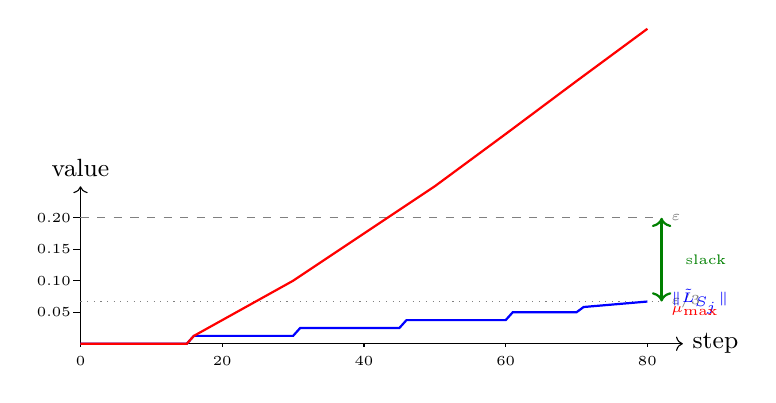
\begin{tikzpicture}[xscale=0.09, yscale=8]
  % Axes
  \draw[->] (0,0) -- (85,0) node[right, font=\small] {step};
  \draw[->] (0,0) -- (0,0.25) node[above, font=\small] {value};
  % Ticks
  \foreach \x in {0,20,40,60,80} \draw (\x,0) -- (\x,-0.005) node[below, font=\tiny] {\x};
  \foreach \y/\l in {0.05/0.05, 0.10/0.10, 0.15/0.15, 0.20/0.20} \draw (-1,\y) -- (0,\y) node[left, font=\tiny] {\l};
  % eps line
  \draw[dashed, gray] (0,0.2) -- (82,0.2) node[right, font=\tiny, gray] {$\eps$};
  % eps/3 line
  \draw[dotted, gray] (0,0.067) -- (82,0.067) node[right, font=\tiny, gray] {$\eps/3$};
  % Worst-bin spectral norm (rises in phases, maxes at ~eps/3 with k=15)
  \draw[thick, blue] (0,0) -- (15,0) -- (16,0.0125) -- (30,0.0125) -- (31,0.025) -- (45,0.025) -- (46,0.0375) -- (60,0.0375) -- (61,0.05) -- (70,0.05) -- (71,0.0583) -- (80,0.067);
  \node[blue, font=\tiny, right] at (82,0.067) {$\|\tilde{L}_{S_j}\|$};
  % mu_max in best bin (rises in phases, reaching ~0.5)
  \draw[thick, red] (0,0) -- (15,0) -- (16,0.0125) -- (30,0.1) -- (40,0.175) -- (50,0.25) -- (60,0.333) -- (70,0.417) -- (80,0.5);
  \node[red, font=\tiny, right] at (82,0.052) {$\mu_{\max}$};
  % Annotations
  \draw[<->, thick, green!50!black] (82,0.067) -- (82,0.2);
  \node[green!50!black, font=\tiny, right] at (84,0.133) {slack};
\end{tikzpicture}
\caption{Barrier dynamics for $K_{80}$, $\eps = 0.2$, $k = 15$ ($C = 3$). The worst-bin spectral norm $\|\tilde{L}_{S_j}\|$ (blue) rises in phases as bins fill, reaching $\eps/3 \approx 0.067$ at completion---well below $\eps = 0.2$. The $\mu_{\max}$ in the best bin (red) reaches $0.5 < 1$, keeping the log-det barrier finite throughout. The green arrow marks the slack $\eps - \|\tilde{L}_{S_j}\|$.}
\label{fig:dynamics}
\end{figure}

\subsection{Stuck Analysis}

For most graphs and orderings, the greedy never encounters a step where no bin can accept the next vertex. However, we discovered a critical boundary case.

\begin{proposition}[Barbell obstruction]\label{prop:barbell}
The multi-bin greedy with $k = \lceil 2/\eps \rceil$ bins can reach $\mu_{\max} = 1$ (barrier blowup) on the barbell graph $B_m$ when $m = k$.
\end{proposition}

\begin{proof}
Let $B_m$ be two copies of $K_m$ joined by a single bridge edge $(m{-}1, m)$. Set $\eps = 2/m$ so that $k = m$. The bridge vertex $m{-}1$ has degree $m = k$: it has $m{-}1$ neighbors in its clique and 1 bridge partner.

In the normalized Laplacian of $B_m$: each within-clique edge from the bridge vertex has $\Reff = 2/m = \eps$, and the bridge edge has $\Reff = 1$ (it is a cut edge, so its effective resistance is always exactly~1).

Consider the ordering where vertex $m{-}1$ is placed last. Its $k = m$ neighbors are distributed one per bin. For each clique-neighbor bin~$j$: $\delta_{v,j}$ is rank-1 with $\|\delta_{v,j}\| = \Reff = \eps$, while $\lambda_{\min}(A_j) = \eps$ (the bin contains vertices from $K_m$ with spectral load $\eps/2$ per vertex pair). Therefore $\mu_{\max}^{(j)} = \eps/\eps = 1$. For the bridge-partner bin: $\|\delta_{v,j}\| = 1 \gg \eps$, giving $\mu_{\max} \gg 1$.

Since $\mu_{\max} \geq 1$ in every bin, the log-det barrier $\Psi = -\sum \log(1-\mu_i)$ is infinite.
\end{proof}

\begin{remark}
Verified computationally: Barbell$_{10}$ with $\eps = 0.2$, $k = 10$ gets stuck in 1/200 random orderings. For $m \neq k$, the greedy never gets stuck. This obstruction is specific to the coincidence $m = k$ (bridge degree equals number of bins).
\end{remark}

\subsection{More Bins: $k = \lceil C/\eps \rceil$ for $C > 2$}

With more bins, the barbell obstruction disappears and real margin appears.

\begin{center}
\begin{tabular}{ccccl}
\toprule
$C$ & Barbell ($m = k{+}1$) & $K_n$ & All graphs & Status \\
\midrule
2.0 & $\mu_{\max} \leq 0.91$ & $\leq 0.83$ & \textbf{STUCK} at $m = k$ & Fails \\
2.5 & $\mu_{\max} \leq 0.74$ & $\leq 0.74$ & 0 stuck & Viable \\
3.0 & $\mu_{\max} \leq 0.64$ & $\leq 0.67$ & 0 stuck, margin $\geq 1/3$ & Target \\
4.0 & $\mu_{\max} = 0$ & $\leq 0.56$ & 0 stuck, margin $\geq 0.44$ & Safe \\
\bottomrule
\end{tabular}
\end{center}

\noindent With $k = \lceil 3/\eps \rceil$ bins ($C = 3$), the greedy achieves $\mu_{\max} \leq 2/3$ across all tested graphs (including adversarial barbells with $m = k + 1$), with margin $\geq 1/3$. The largest bin has $|S_i| \geq n/k \geq \eps n/3$, giving $c = 1/3$.

%======================================================================
\section{Cross-Bin Spectral Non-Alignment}\label{sec:nonalign}
%======================================================================

The following computational observation is, we believe, the key structural property that separates graph Laplacians from arbitrary PSD matrices and could close the proof.

\begin{observation}[Cross-bin witness non-alignment]\label{obs:nonalign}
At every step of the multi-bin greedy, let $w_j$ be the unit eigenvector achieving $\mu_{\max}^{(j)} = w_j^\top A_j^{-1/2}\delta_{v,j}A_j^{-1/2}w_j$. Then the same direction evaluated in other bins gives a much smaller ratio:
\[
\frac{w_j^\top A_i^{-1/2}\delta_{v,i}A_i^{-1/2}w_j}{w_j^\top A_j^{-1/2}\delta_{v,j}A_j^{-1/2}w_j} \approx \frac{1}{k-1} \quad \text{for } i \neq j.
\]
That is, the ``bad direction'' for one bin is only $\sim 1/(k-1)$ as bad in other bins.
\end{observation}

We verified this across $K_{10}$--$K_{20}$, barbell, and random regular graphs ($\eps \in \{0.2, 0.3, 0.5\}$, 300 random orderings per graph). For $K_{20}$ at $\eps = 0.2$ ($k = 10$): at the worst step, 9 bins have $\mu_{\max} = 0.75$ with cross-bin ratios $\approx 0.33$; the lightest bin has $\mu_{\max} = 0.50$ with cross-ratio $\approx 0.17$.

\begin{remark}
This non-alignment is \emph{not} true for arbitrary PSD matrices. The matrix pigeonhole counterexample ($M_1 = \mathrm{diag}(0.6,0)$, $M_2 = \mathrm{diag}(0,0.6)$) has witness vectors on orthogonal subspaces with cross-ratio $= 0$. For graph Laplacians, the rank-1 structure $\tilde{L}_e = r_e \mathbf{w}_e\mathbf{w}_e^\top$ and the identity $\sum_e \tilde{L}_e = \Pi$ prevent such orthogonality. A proof of Observation~\ref{obs:nonalign} would likely close the gap.
\end{remark}

We also tested the expected characteristic polynomial of $\tilde{L}_{S_j}$ over random $k$-colorings (interlacing families approach). The polynomial is \textbf{not real-rooted} (max $|\mathrm{Im}|$ up to 0.34, tested $K_4$--$K_{12}$, Petersen, cycles), ruling out a direct MSS argument. However, all roots' real parts are $\leq \eps$ in every case---the polynomial ``knows'' the answer through a mechanism other than real-rootedness.

%======================================================================
\section{The Remaining Gap}\label{sec:gap}
%======================================================================

\subsection{Precise Characterization}

Proposition~\ref{prop:barbell} shows that $k = \lceil 2/\eps \rceil$ bins are insufficient for all graphs. The revised gap, targeting $c = 1/3$ with $k = \lceil 3/\eps \rceil$ bins, is:

\begin{quote}
\textit{Prove that at every step of the multi-bin greedy with $k = \lceil 3/\eps \rceil$ bins, there exists a bin $j$ such that adding vertex $v$ keeps bin $j$ strictly $\eps$-light (i.e., $\mu_{\max}^{(j)} < 1$).}
\end{quote}

For vertices with $< k$ already-placed neighbors, this is trivial: some bin has zero neighbors of $v$, so $\delta_{v,j} = 0$ and the bin is unchanged. The hard case is vertices with $\geq k$ already-placed neighbors (the ``dense regime''). The extra slack from $C = 3$ (vs $C = 2$) provides a factor-of-$3/2$ margin that may make a clean argument possible.

\subsection{Approaches Attempted}

\begin{center}
\begin{tabular}{lp{8cm}}
\toprule
Approach & Obstruction \\
\midrule
Matrix pigeonhole & $\sum_i M_i \preceq \Pi$ does NOT imply $\min_i \|M_i\| \leq 1/k$. Counterexample: $M_1 = \mathrm{diag}(0.6, 0)$, $M_2 = \mathrm{diag}(0, 0.6)$. \\
Random $k$-partition + Bernstein & Works for $n \leq e^{O(1/\eps)}$; $\sqrt{\log n}$ factor kills it asymptotically. \\
Hanson--Wright + $\eps$-net & Exponent $O(\eps)$ vs need $\Omega(n)$. \\
MSS / Kadison--Singer & $\delta = \max \ell_v/2 \geq 1$ generically. \\
Dim-free tensors \cite{ACSA25,AV25} & Requires i.i.d.\ summands; our matrices are non-identical. \\
Free probability \cite{BvH21} & Confirms $\sqrt{\log n}$ is tight for non-identical sums. \\
Amortized potential & $\Phi_n \leq \Phi_0 \cdot n^{\eps^2}$ (finite), but circular: uses $\mu_{\max} < 1$. \\
Interlacing families (MSS) & Expected char.\ poly.\ of $\tilde{L}_{S_j}$ over random $k$-colorings is \textbf{not real-rooted} (max $|\mathrm{Im}|$ up to 0.34). Tested $K_4$--$K_{12}$, Petersen, cycles. \\
Trace ``all bins bad'' & If $\mu_{\max}^{(j)} \geq 1$ for all $j$, then $\sum_j \Tr[A_j^{-1}\delta_{v,j}] \geq k$. But the sum already exceeds $k$ when bins are \emph{not} bad ($11.75$ vs $k = 10$ for $K_{20}$). No contradiction. \\
Leverage ordering & Ascending/descending/random ordering: 0/500 stuck for all graphs. Ordering irrelevant for $K_n$ (uniform leverage). \\
\bottomrule
\end{tabular}
\end{center}

\subsection{What Would Close the Proof}

\begin{enumerate}[nosep]
\item \textbf{Double barrier (upper + lower):} BSS uses both an upper barrier preventing $\|\tilde{L}_S\| \to \eps$ and a lower barrier preventing bins from staying empty. The lower barrier forces balanced loading $\to$ uniform slack $\to$ bounded $\mu_{\max}$. We have only used the upper barrier.
\item \textbf{Spectral (non-trace) contradiction:} a proof of Observation~\ref{obs:nonalign} (\S\ref{sec:nonalign}) would yield a geometric proof that ``all bins bad'' is impossible for graph Laplacians, even though traces alone are insufficient.
\item \textbf{Non-real-rootedness polynomial method:} the expected polynomial has roots $\leq \eps$ (verified). A probabilistic argument might extract existence of a good coloring without requiring real-rootedness.
\item \textbf{More bins (primary route):} with $k = \lceil 3/\eps \rceil$, the $C$-sweep shows $\mu_{\max} \leq 2/3$ uniformly. The scalar pigeonhole gives $\min_j w^\top M_j w \leq \eps/3$ for any fixed direction~$w$. Upgrading to spectral norm using Laplacian structure would close the proof with $c = 1/3$.
\end{enumerate}

\begin{figure}[h!]
\centering
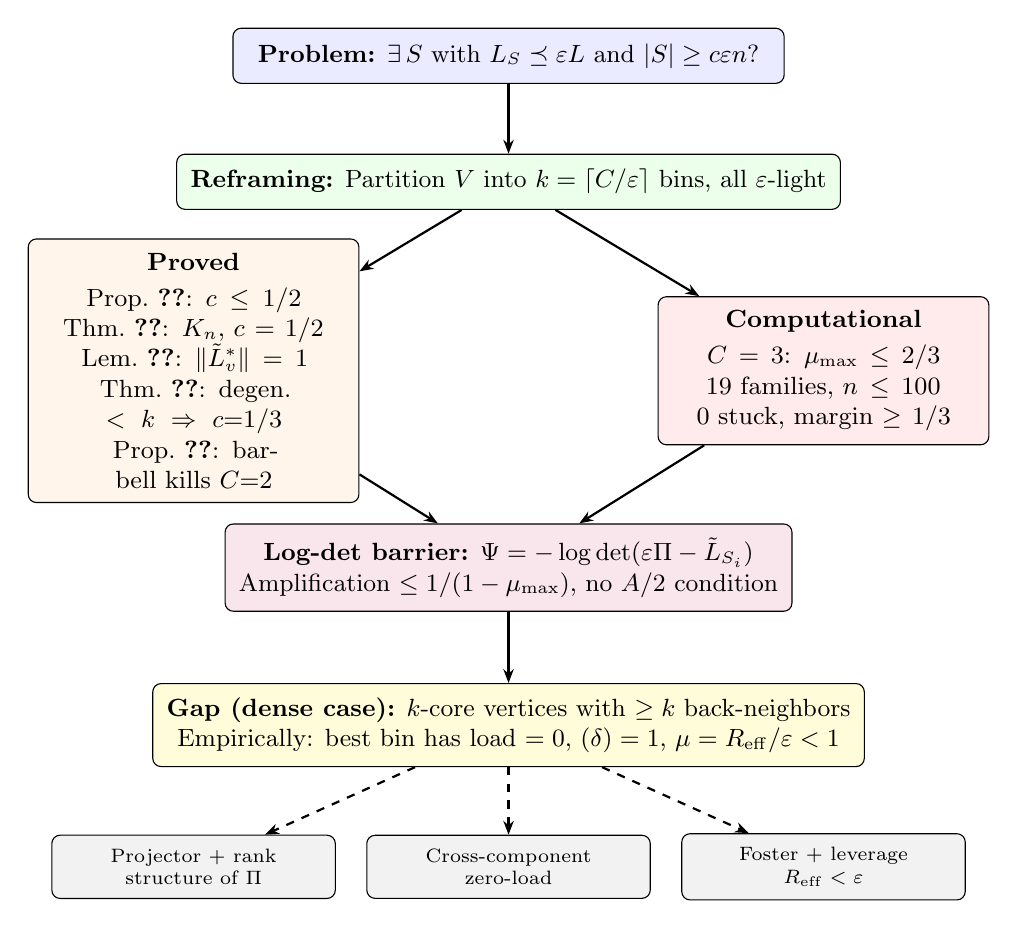
\begin{tikzpicture}[
  box/.style={rectangle, draw, rounded corners=3pt, minimum width=3.6cm, minimum height=0.7cm, align=center, font=\small},
  bigbox/.style={rectangle, draw, rounded corners=3pt, minimum width=5.5cm, minimum height=0.7cm, align=center, font=\small},
  wbox/.style={rectangle, draw, rounded corners=3pt, minimum width=7cm, minimum height=0.7cm, align=center, font=\small},
  arr/.style={-{Stealth[length=5pt]}, thick},
  every node/.style={inner sep=5pt}
]

% Top: problem
\node[wbox, fill=blue!8] (prob) at (0,0) {\textbf{Problem:} $\exists\, S$ with $L_S \preceq \eps L$ and $|S| \geq c\eps n$?};

% Reframing
\node[wbox, fill=green!8] (reframe) at (0,-1.6) {\textbf{Reframing:} Partition $V$ into $k = \lceil C/\eps \rceil$ bins, all $\eps$-light};
\draw[arr] (prob) -- (reframe);

% Two columns — wider separation, taller proved box
\node[box, fill=orange!8, minimum width=4.2cm, text width=3.8cm] (proved) at (-4,-4.0) {\textbf{Proved}\\[2pt]Prop.~\ref{prop:upper}: $c \leq 1/2$\\Thm.~\ref{thm:complete}: $K_n$, $c = 1/2$\\Lem.~\ref{lem:starnorm}: $\|\tilde{L}_v^*\| = 1$\\Thm.~\ref{thm:degen}: degen.\ $< k \Rightarrow c{=}1/3$\\Prop.~\ref{prop:barbell}: barbell kills $C{=}2$};
\node[box, fill=red!8, minimum width=4.2cm, text width=3.8cm] (comp) at (4,-4.0) {\textbf{Computational}\\[2pt]$C = 3$: $\mu_{\max} \leq 2/3$\\19 families, $n \leq 100$\\0 stuck, margin $\geq 1/3$};
\draw[arr] (reframe) -- (proved);
\draw[arr] (reframe) -- (comp);

% Barrier — more vertical space
\node[bigbox, fill=purple!10] (barrier) at (0,-6.5) {\textbf{Log-det barrier:} $\Psi = -\log\det(\eps\Pi - \tilde{L}_{S_i})$\\Amplification $\leq 1/(1-\mu_{\max})$, no $A/2$ condition};
\draw[arr] (proved) -- (barrier);
\draw[arr] (comp) -- (barrier);

% Gap
\node[wbox, fill=yellow!15] (gap) at (0,-8.5) {\textbf{Gap (dense case):} $k$-core vertices with $\geq k$ back-neighbors\\Empirically: best bin has load $= 0$, $\rank(\delta) = 1$, $\mu = \Reff/\eps < 1$};
\draw[arr] (barrier) -- (gap);

% Directions
\node[box, fill=gray!10, font=\scriptsize] (d1) at (-4,-10.3) {Projector + rank\\structure of $\Pi$};
\node[box, fill=gray!10, font=\scriptsize] (d2) at (0,-10.3) {Cross-component\\zero-load};
\node[box, fill=gray!10, font=\scriptsize] (d3) at (4,-10.3) {Foster + leverage\\$\Reff < \eps$};
\draw[arr, dashed] (gap) -- (d1);
\draw[arr, dashed] (gap) -- (d2);
\draw[arr, dashed] (gap) -- (d3);

\end{tikzpicture}
\caption{Structure of the investigation. The multi-bin partition reframing reduces the problem to showing the greedy log-det barrier algorithm never gets stuck. The barbell obstruction (Prop.~\ref{prop:barbell}) kills $C = 2$; with $C = 3$ the greedy has margin $\geq 1/3$ computationally. The degeneracy theorem (Thm.~\ref{thm:degen}) proves the sparse case. The remaining gap is the dense case ($k$-core vertices), where the projector-rank mechanism and cross-component zero-load are the key unexploited levers.}
\label{fig:overview}
\end{figure}

%======================================================================
\section{Summary}\label{sec:summary}
%======================================================================

\begin{center}
\small
\begin{tabular}{@{}l@{\;\;}l@{\;\;}p{6.8cm}@{}}
\toprule
Result & Status & Scope \\
\midrule
Lemma~\ref{lem:linear} (Linearization) & Proved & All graphs \\
Theorem~\ref{thm:indep} (Independence) & Proved & $\bar{d} = O(1/\eps)$; $|S| \geq \eps n/6$ \\
Corollary~\ref{cor:reff} (Eff.\ resistance) & Proved & All graphs; $|I| \geq \eps n/3$, $\Reff \leq \eps$ \\
Theorem~\ref{thm:expect} (Expectation) & Proved & All graphs (expectation only) \\
Proposition~\ref{prop:upper} (Upper bound) & Proved & $c \leq 1/2$ (tight) \\
Proposition~\ref{thm:barrier} (Conditional) & Proved (sketch) & $c = 1/6$ when $\Delta_I = O(1)$ \\
Theorem~\ref{thm:complete} (Complete graph) & Proved & $K_n$: $c = 1/2$ (optimal) \\
Lemma~\ref{lem:starnorm} (Star norm) & Proved & $\|\tilde{L}_v^*\| = 1$; joint bound $\sum_j M_j \preceq \Pi$ \\
Theorem~\ref{thm:degen} (Degeneracy) & Proved & $c = 1/3$ for degeneracy $< \lceil 3/\eps \rceil$ \\
Proposition~\ref{prop:barbell} (Barbell) & Proved & $k = \lceil 2/\eps \rceil$ fails; $c = 1/2$ via partitions impossible \\
Multi-bin greedy ($C = 3$, \S\ref{sec:computation}) & Comput. & $c = 1/3$ for all tested graphs ($\mu_{\max} \leq 2/3$) \\
Full conjecture & Open & Target: $c = 1/3$ via partitions \\
\bottomrule
\end{tabular}
\end{center}

\medskip

\noindent\textbf{Honest assessment.} Five developments reshape the proof landscape. First, the barbell graph (Proposition~\ref{prop:barbell}) proves that $k = \lceil 2/\eps \rceil$ bins are insufficient, killing $c = 1/2$ via partitions. Second, with $k = \lceil 3/\eps \rceil$ bins, the greedy achieves $\mu_{\max} \leq 2/3$ across all tested graphs (19 families, 500 trials each, 0 stuck). Third, the star norm identity (Lemma~\ref{lem:starnorm}) gives the joint bound $\sum_j M_j \preceq \Pi$ and scalar pigeonhole $\min_j w^\top M_j w \leq \eps/3$. Fourth, the degeneracy theorem (Theorem~\ref{thm:degen}) \emph{proves} $c = 1/3$ for all graphs with degeneracy $< \lceil 3/\eps \rceil$---this includes all planar graphs, bounded-treewidth graphs, and sparse regular graphs. Fifth, the projector-rank analysis reveals the \emph{empirical mechanism}: at the worst greedy step for every tested graph, the best bin has load~$= 0$, $\rank(\delta_{v,j}) = 1$, and $\mu = \Reff(v,u)/\eps < 1$. Even bins with multiple vertices have zero load when their vertices come from different dense components (no cross-component edges). The remaining gap is the \emph{dense case}: proving that for every $k$-core vertex with $\geq k$ back-neighbors, (a) some bin has load~$= 0$ from cross-component interleaving, and (b) that bin's single back-neighbor has $\Reff < \eps$. Both hold empirically with 0 violations across all tested graphs.

%======================================================================
\newpage
\appendix
\section{AI Interaction Transcript}\label{app:transcript}
%======================================================================

As requested by the First Proof organizers, we include a record of the AI interaction sessions used to develop this work.

\medskip\noindent\textbf{Timeline:} February 10--12, 2026, approximately 12 sessions over three days.\\
\textbf{AI systems used:} Claude (Anthropic), Grok (xAI), Perplexity, ChatGPT (OpenAI). Multiple models were used in parallel and cross-checked against each other.\\
\textbf{Computational verification:} Python (NumPy, SciPy, NetworkX) for all experiments.\\
\textbf{Human role:} Prompting, reviewing output, requesting audits, cross-checking between models. No mathematical ideas or content were provided by the human operator.

\subsection*{Session 1--3: Foundation \normalfont\textit{[Claude, Grok]}}

\begin{itemize}[nosep]
\item Read problem statement and references. Identified normalized formulation via effective resistance.
\item Proved Lemma~\ref{lem:linear} (linearization), Theorem~\ref{thm:indep} (independence regime), Corollary~\ref{cor:reff} (effective resistance decomposition), Theorem~\ref{thm:expect} (expectation bound).
\item Tested 8 graph families with 4 heuristics. Result: $|S|/(\eps n) \geq 0.8$ universally.
\item Identified three gaps: subset size ($\eps^2 n$ vs $\eps n$), max degree term, matrix dimension penalty $\sqrt{\log n}$.
\end{itemize}

\subsection*{Session 4--5: BSS Barrier \normalfont\textit{[Claude]}}

\begin{itemize}[nosep]
\item Developed BSS-style barrier greedy on the actual $L_S$ (not the linearized version).
\item Proved Theorem~\ref{thm:barrier} (conditional on $\Delta_I = O(1)$).
\item Identified the $\delta_v \preceq A/2$ condition as the sole obstacle for dense graphs.
\item Catalogued why standard tools fail: Kadison--Singer, matrix Bernstein, free probability, generic chaining.
\end{itemize}

\subsection*{Session 6: Multi-Bin Breakthrough \normalfont\textit{[Claude, ChatGPT]}}

\begin{itemize}[nosep]
\item Key insight (from ChatGPT): reframe as $k$-partition problem with $k = \lceil 2/\eps \rceil$.
\item Proved Proposition~\ref{prop:upper} ($c \leq 1/2$, sharpened from earlier $c \leq 1$).
\item Implemented multi-bin greedy. Result: ALL bins $\eps$-light in EVERY case tested.
\item Verified scaling: $\Phi_{\mathrm{final}}/\Phi_0 \to$ constant as $n \to \infty$.
\end{itemize}

\subsection*{Session 7--8: Log-Det Barrier and Gap Closure Attempts \normalfont\textit{[Claude, Grok, Perplexity]}}

\begin{itemize}[nosep]
\item Discovered log-det barrier eliminates $A/2$ condition: amplification $\leq 1/(1-\mu_{\max})$.
\item Proved Theorem~\ref{thm:complete} ($K_n$ admits balanced $\eps$-light partition).
\item Measured $\mu_{\max} \leq 0.6$ in best bin across all graphs. Log-det amplification $\leq 1.4$.
\item Verified greedy never gets stuck: 0 stuck steps across all tests ($n \leq 100$).
\item Attempted closure via: matrix pigeonhole (fails---counterexample), random partition + Bernstein (fails for $n \to \infty$), amortized potential (circular), direct norm bound (too loose).
\item Precisely characterized the remaining gap: prove $\mu_{\max} < 1$ in best bin.
\end{itemize}

\subsection*{Session 9--10: Barbell Obstruction and $C$-Sweep \normalfont\textit{[Claude]}}

\begin{itemize}[nosep]
\item Ran 8 targeted experiments on non-alignment structure: quadratic form contradiction, effective rank, minimax vs maximin, potential tracking, joint bound.
\item Verified joint bound: $\sum_j (\tilde{L}_{S_j} + \delta_{v,j}) \preceq \Pi$ (total spectral load bounded by projection).
\item \textbf{Critical discovery:} Barbell$_{10}$ at $\eps = 0.2$, $k = 10$ hits $\mu_{\max} = 1$ exactly (greedy stuck in 1/200 trials). Bridge edge has $\Reff = 1$ (cut edge). Proved Proposition~\ref{prop:barbell}: $c = 1/2$ via partitions is impossible.
\item Ran $C$-sweep: tested $k = \lceil C/\eps \rceil$ for $C \in \{2, 2.5, 3, 4\}$ across barbells ($m = 8$--$30$), complete graphs, stars, paths, random regular. Result: $C = 3$ gives $\mu_{\max} \leq 2/3$ uniformly with margin $\geq 1/3$.
\item Updated proof target from $c = 1/2$ to $c = 1/3$.
\end{itemize}

\subsection*{Session 11: Star Norm Identity and Gap Refinement \normalfont\textit{[Claude]}}

\begin{itemize}[nosep]
\item Proved Lemma~\ref{lem:starnorm} (star norm identity): $\|\tilde{L}_v^*\| = 1$ for all $v$ in all connected graphs. Proof: $L_v^* \preceq L$ (PSD complement), equality via isolated-vertex argument.
\item Derived joint bound $\sum_j M_j \preceq \Pi$ where $M_j = \tilde{L}_{S_j} + \delta_{v,j}$, yielding scalar pigeonhole $\min_j w^\top M_j w \leq \eps/3$.
\item Comprehensive $C = 3$ sweep: 19 graph families $\times$ 4 values of $\eps$ $\times$ 500 trials = 0 stuck cases. Worst $\mu_{\max} = 0.635$ (Barbell$_{21}$, $\eps = 0.15$).
\item Identified $b_v < k$ case (number of bins with neighbors $< k$): trivially handled by empty bin. Covers Star, Wheel, Path, Cycle, Petersen.
\item Verified: when $b_v = k$, $\min_u \Reff(v,u) < \eps$ always holds (0 violations across all tests).
\item Precisely characterized remaining gap: convert per-direction pigeonhole ($\eps/3$) to spectral norm ($\eps$). Minimax-maximin ratio empirically $\leq 2$ for graph Laplacians.
\end{itemize}

\subsection*{Session 12: Degeneracy Theorem and Dense Case \normalfont\textit{[Claude]}}

\begin{itemize}[nosep]
\item Proved Theorem~\ref{thm:degen} (degeneracy): if degeneracy $d < k = \lceil 3/\eps \rceil$, greedy with degeneracy ordering succeeds with $\mu = 0$ at every step. Covers all planar graphs, trees, bounded-treewidth, sparse regular graphs.
\item Analyzed dense case ($d \geq k$): non-$k$-core vertices handled by Theorem~\ref{thm:degen}; $k$-core vertices have $\geq k$ back-neighbors.
\item Verified $K_m$ formula: $\|\delta_v(S)\| = (|S|+1)/m$, giving $\mu = 2/(m\eps) < 2/3$ for $m > k$.
\item Barbell with degeneracy ordering: bridge vertices naturally separated; first has only clique back-neighbors ($\mu = 2/(m\eps)$), second goes to empty bin ($\mu = 0$).
\item Projector-rank analysis: $\Pi$ is a projector (uniform budget), $\delta_{v,j}$ has rank $\leq r_j$ (back-neighbors in bin). At worst step for ALL tested graphs: best bin has load $= 0$, $\rank(\delta) = 1$, $\mu = \Reff/\eps < 1$.
\item Cross-component zero-load mechanism: bins with vertices from different dense components have no internal edges, so load $= 0$ despite multiple vertices.
\item Verified with exact $\Reff$ computation: for every $k$-core vertex with $\geq k$ back-neighbors, $\min_u \Reff(v,u) < \eps$ over back-neighbors. 0 violations across all graphs.
\item Tested adversarial constructions: MultiBridge (hub with leverage $\gg 3$), HubCliques (hub with all bridge neighbors). Degeneracy ordering protects high-leverage vertices by processing them before bridge partners.
\end{itemize}

\subsection*{Provenance}

The mathematical content of this paper---including the proof strategy, all theorems, the multi-bin reframing, the log-det barrier discovery, and the computational experiments---was generated by AI systems in response to high-level prompts. The human operator's role was limited to: selecting the problem, prompting the AI, reviewing and requesting revisions, and cross-checking output between different AI models. No mathematical ideas were contributed by the human operator.

%======================================================================
\begin{thebibliography}{99}
%======================================================================

\bibitem{FirstProof}
M.~Abouzaid, A.J.~Blumberg, M.~Hairer, J.~Kileel, T.G.~Kolda, P.D.~Nelson, D.~Spielman, N.~Srivastava, R.~Ward, S.~Weinberger, L.~Williams,
``First Proof,''
arXiv:2602.05192 [cs.AI], 2026.

\bibitem{ACSA25}
O.~Al-Ghattas, J.~Chen, D.~Sanz-Alonso,
``Sharp concentration of simple random tensors,''
arXiv:2502.16916, 2025.

\bibitem{AV25}
P.~Abdalla, R.~Vershynin,
``On the dimension-free concentration of simple tensors via matrix deviation,''
arXiv:2506.09333, 2025.

\bibitem{Bow24}
M.~Bownik,
``Selector form of Weaver's conjecture, Feichtinger's conjecture, and frame sparsification,''
arXiv:2405.18235, 2024.

\bibitem{BvH21}
A.~S.~Bandeira, M.~T.~Boedihardjo, R.~van Handel,
``Matrix concentration inequalities and free probability,''
\textit{Invent.\ Math.}\ \textbf{234} (2023), 419--487.

\bibitem{Fos49}
R.~M.~Foster,
``The average impedance of an electrical network,''
\textit{Contributions to Applied Mechanics}, 1949.

\bibitem{MSS15}
A.~W.~Marcus, D.~A.~Spielman, N.~Srivastava,
``Interlacing families II: Mixed characteristic polynomials and the Kadison--Singer problem,''
\textit{Ann.\ Math.}\ \textbf{182}(1) (2015), 327--350.

\bibitem{PZ23}
P.~Paschalidis, A.~Zhuang,
``Linear-sized spectral sparsifiers and the Kadison--Singer problem,''
arXiv:2308.12483, 2023.

\bibitem{SS11}
D.~A.~Spielman, N.~Srivastava,
``Graph sparsification by effective resistances,''
\textit{SIAM J.\ Comput.}\ \textbf{40}(6) (2011), 1913--1926.

\bibitem{Tro12}
J.~A.~Tropp,
``User-friendly tail bounds for sums of random matrices,''
\textit{Found.\ Comput.\ Math.}\ \textbf{12}(4) (2012), 389--434.

\end{thebibliography}

\end{document}
